\section{Results}
In this section we will show the results that we get for the 3 materials. We
will compare the results we get with our 3D code and CEPXS/ONELD, which is a
1D code. 
\subsection{Water}
For this example, we are using a $S_{12}$ Galerkin-Legendre-Chebyshev
quadrature. The medium is 20 cm thick and there is an incoming flux of
photons. The source of photons has an energy of 1MeV ans we use a cut-off
energy of 0.01MeV. Thus, every particles which has an energy lower than 
0.01 MeV is assumed to depose all its energy without moving anymore.
\subsection{Aluminium}
For this example, we are using a $S_{12}$ Galerkin Gauss-Legendre-Chebyshev 
quadrature. The medium is 5cm thick and there is an incoming flux of photons.
The source of photons has an energy of 20 MeV and we use a cut-off energy of
0.01 MeV.\\
In the following table, we show the dose computed every centimeter using
different scattering order :
\begin{table}[H]
\begin{center}
\begin{tabular}{|c|c|c|c|c|c|}
\hline
Position & order = 13 & order = 11 & order = 9 & order = 7 & order = 5 \\
\hline
0 & 0.0146404 & 0.0146402 & 0.0141156 & 0.0166718 & 0.0087276 \\
1 & 0.1697907 & 0.1697890 & 0.1698012 & 0.1695422 & 0.1728969 \\
2 & 0.2752749 & 0.2752729 & 0.2753298 & 0.2742052 & 0.2775113 \\
3 & 0.3161310 & 0.3161307 & 0.3165279 & 0.3145572 & 0.3199176 \\
4 & 0.3120572 & 0.3120566 & 0.3125514 & 0.3104412 & 0.3153226 \\
5 & 0.2087631 & 0.2087634 & 0.2094064 & 0.2061794 & 0.2154810 \\
\hline
\end{tabular}
\caption{Dose : $\frac{MeV}{g}$}
\end{center}
\end{table}     
We can see that if we except the border of the domain, the results obtained by
using a $P_5$ order for the scattering are very closed to the one using the
full order. The reason is that the high-order moment are very small :
               
\begin{figure}[H]
\begin{minipage}[b]{0.45\linewidth}
\centering
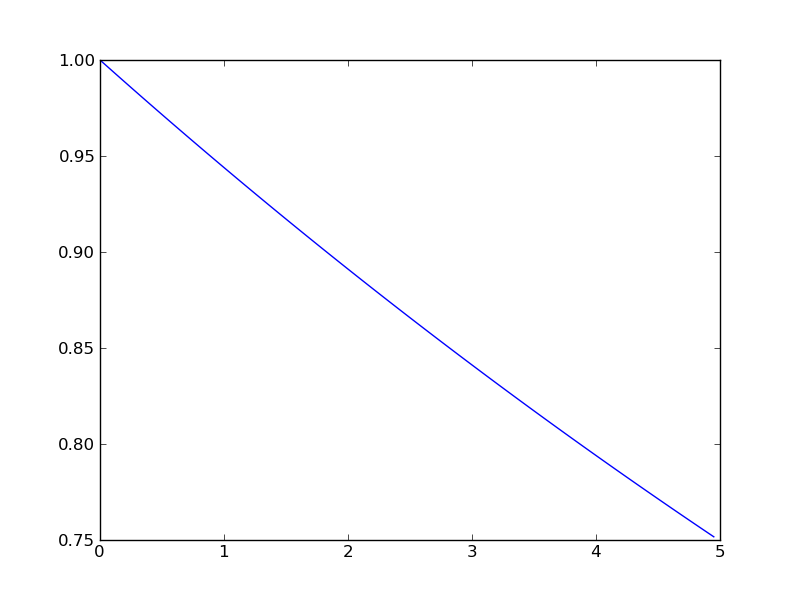
\includegraphics[width=\linewidth]{./images/al/group_0_moment_0}
\caption{$Y_0^0$ first photon group}
\end{minipage}
\hspace{0.5cm}
\begin{minipage}[b]{0.45\linewidth}
\centering
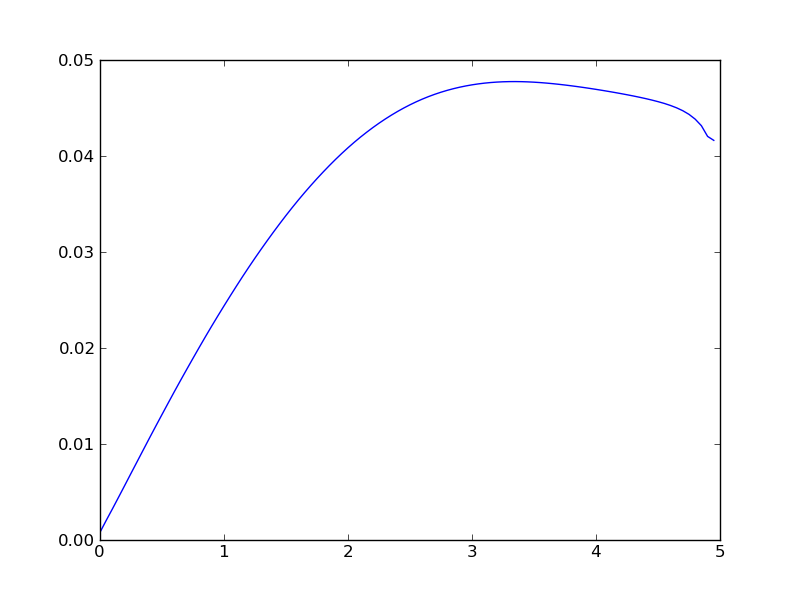
\includegraphics[width=\linewidth]{./images/al/group_39_moment_0}
\caption{$Y_0^0$ last electron group}
\end{minipage}
\end{figure}

\begin{figure}[H]
\begin{minipage}[b]{0.45\linewidth}
\centering
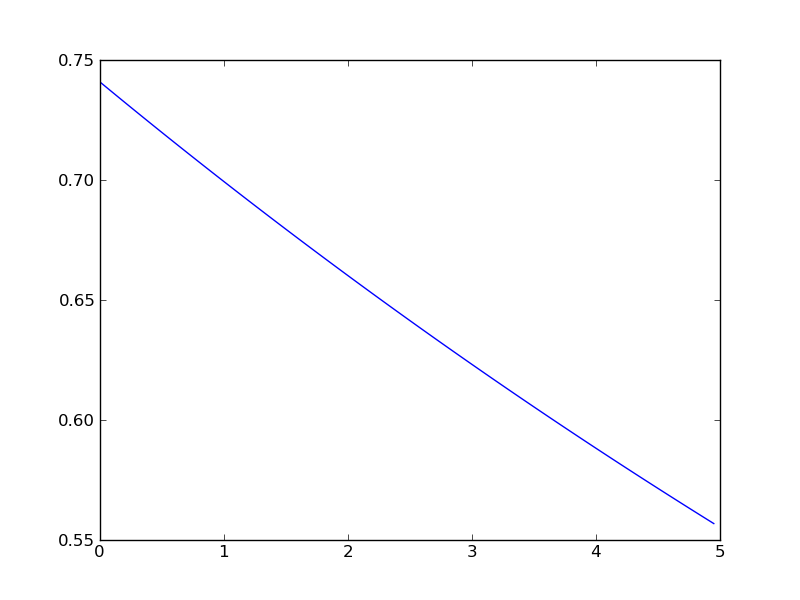
\includegraphics[width=\linewidth]{./images/al/group_0_moment_30}
\caption{$Y_5^0$ first photon group}
\end{minipage}
\hspace{0.5cm}
\begin{minipage}[b]{0.45\linewidth}
\centering
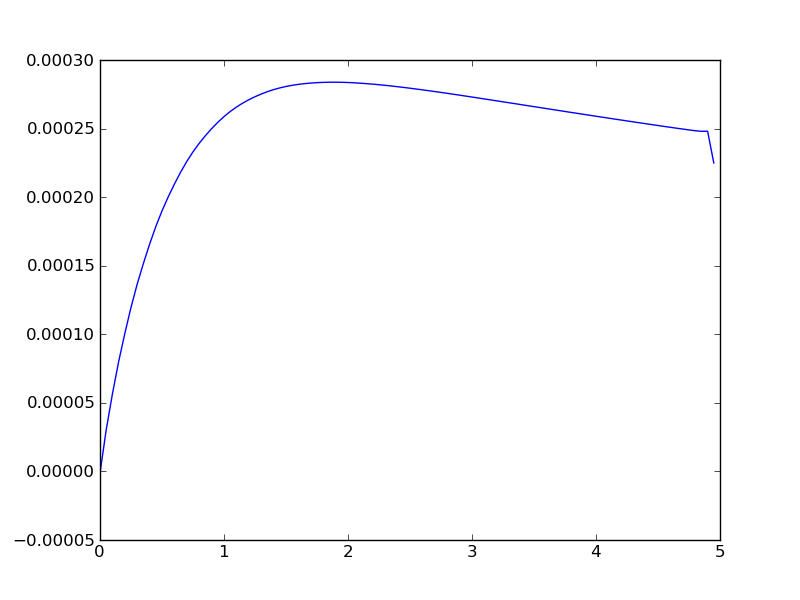
\includegraphics[width=\linewidth]{./images/al/group_39_moment_30}
\caption{$Y_5^0$ last electron group}
\end{minipage}
\end{figure}

\begin{figure}[H]
\begin{minipage}[b]{0.45\linewidth}
\centering
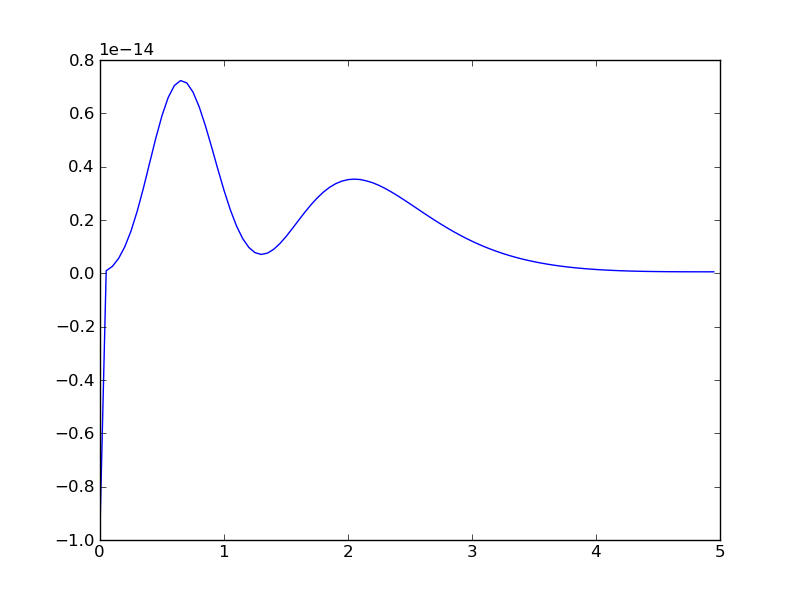
\includegraphics[width=\linewidth]{./images/al/group_0_moment_142}
\caption{$Y_{11}^0$ first photon group}
\end{minipage}
\hspace{0.5cm}
\begin{minipage}[b]{0.45\linewidth}
\centering
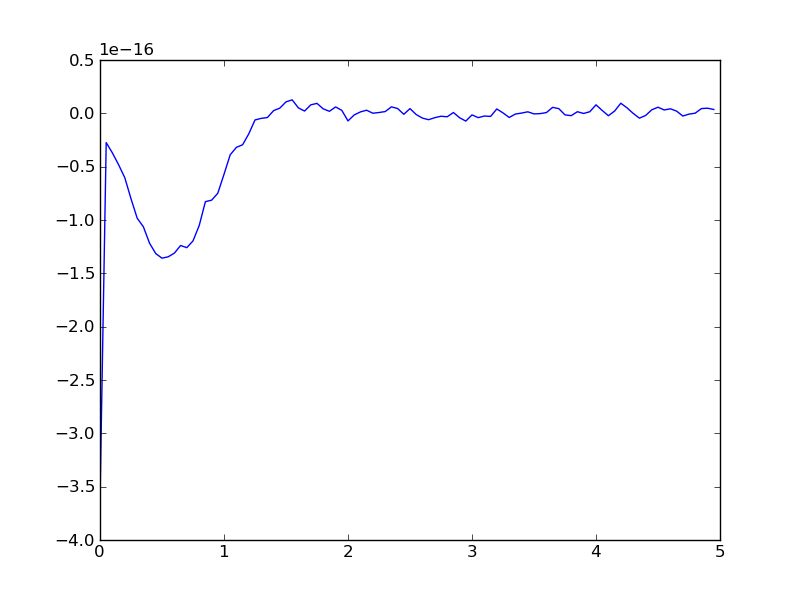
\includegraphics[width=\linewidth]{./images/al/group_39_moment_142}
\caption{$Y_{11}^0$ last electron group}
\end{minipage}
\end{figure}

\subsection{Gold}
The setup of this problem is the same as the previous one. The only difference
is that now the medium is made of gold instead of aluminium.\\
We can see that the results are always very good. Decreasing the order of the
scattering do not change the result significantly.
